% \IUref{IUAdmPS}{Administrar Planta de Selección}
% \IUref{IUModPS}{Modificar Planta de Selección}
% \IUref{IUEliPS}{Eliminar Planta de Selección}


% Copie este bloque por cada caso de uso:
%-------------------------------------- COMIENZA descripción del caso de uso.

%\begin{UseCase}[archivo de imágen]{UCX}{Nombre del Caso de uso}{
	\begin{UseCase}{CU29.0}{Registrar salida de área}{
		En esta sección podrá registrar su salida de una área.
	}
		\UCitem{Versión}{1.0}
		\UCitem{Actor}{Usuario}
		\UCitem{Propósito}{Permitir la salida al usuario que ya no desee permanecer mas tiempo en el área en donde se encuentre.}
		\UCitem{Entradas}{Clave del usuario.}
		\UCitem{Origen}{El dato será ingresado desde un teclado.}
		\UCitem{Salidas}{Mensaje de salida registrada, hora de salida.}
		\UCitem{Destino}{El registro será enviado a la base de datos, de la tabla registrar salida, con el campo salida activado en 1.}
		\UCitem{Precondiciones}{Que el usuario haya ingresado previamente a un área y haya sido identificado correctamete.}
		\UCitem{Postcondiciones}{El usuario no podrá ingresar al área si es que excede su tiempo limite por día.}
		\UCitem{Errores}{Que el sistema no reconozca al usuario identificado y no permita el acceso.}
		\UCitem{Tipo}{Caso de uso primario}
		\UCitem{Observaciones}{Este dato será requerido en la salida de cada área.}
		\UCitem{Autor}{Francisco García Enríquez.}
		\UCitem{Revisor}{Isaac Fernandez.}
	\end{UseCase}

	\begin{UCtrayectoria}{Principal}
		\UCpaso[\UCactor] solicita la salida por medio de una pantalla.
		\UCpaso Muestra un campo con el nombre clave.
		\UCpaso[\UCactor] ingresará su clave.
		\UCpaso[\UCactor] Confirma su salida, presionando el boton salir.
		\UCpaso Muestra un mensaje {\bf MSG21-}``Acceso correcto.'' el cual permanece activo durante 2 segundos.
		\UCpaso permite la salida y abre la puerta.
	\end{UCtrayectoria}
%-------------------------------------- TERMINA descripción del caso de uso.

		\begin{UCtrayectoriaA}{A}{El usuario excede el limite de tiempo en el área.}
			\UCpaso[\UCactor] Confirma su salida, presionando el boton acceder.
			\UCpaso Muestra un mensaje {\bf MSG22-}``Tiempo excedido.'' con una duración de 2 segundos.
			\UCpaso Muestra un mensaje {\bf MSG23-}``Acceso correcto.''  que permanece activo durante 2 segundos.
			\UCpaso Permite la salida y abre la puerta.
		\end{UCtrayectoriaA}

\begin{figure}[htbp!]
		\centering
			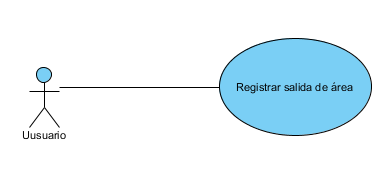
\includegraphics[width=0.8\textwidth]{images/registraSalidaArea}
		\caption{Diagrama de Casos de Uso del sistema.}
	\end{figure}
	